\documentclass[11pt,twocolumn,oneside,openany,headings=optiontotoc,11pt,numbers=noenddot,final]{article}

\usepackage[a4paper]{geometry}
\usepackage[utf8]{inputenc}
\usepackage[T1]{fontenc}
\usepackage{lmodern}
\usepackage[ngerman]{babel}
\usepackage{ngerman}

\usepackage[onehalfspacing]{setspace}

\usepackage{fancyhdr}
\usepackage{fancybox}

\usepackage{rotating}
\usepackage{varwidth}

%Struktogramme
\usepackage[german,curves]{struktex}

\usepackage{pdflscape}
\usepackage{changepage}
\usepackage{graphicx}
\usepackage[bottom]{footmisc}
\usepackage{transparent}
\usepackage{graphbox}
\graphicspath{
	{Pics/PDFs/}
	{Pics/JPGs/}
	{Pics/PNGs/}
}
\usepackage{caption}
\usepackage{wrapfig}
\usepackage{marginnote}
\usepackage{tabularx}
\usepackage{dashrule}
\usepackage{soulutf8}
\usepackage{hhline}
%arydshln suppresses vertical lines in table
%\usepackage{arydshln}
\usepackage{multirow}
\usepackage{enumerate}
\usepackage[hidelinks]{hyperref}
\usepackage{listings}

\usepackage[table]{xcolor}
\usepackage{array}
\usepackage{enumitem,amssymb,amsmath}
\usepackage{interval}
\usepackage{cancel}
\usepackage{stmaryrd}
\usepackage{wasysym}
\usepackage{polynom}
\usepackage{diagbox}
\usepackage{dashrule}
\usepackage{framed}
\usepackage{mdframed}
\usepackage{karnaugh-map}
\usepackage{pdfpages}

\usepackage{blindtext}

\usepackage{eso-pic}

\usepackage{amssymb}
\usepackage{eurosym}

\usepackage[pages=some]{background}
\pagestyle{headings}
\renewcommand{\headrulewidth}{0.2pt}
\renewcommand{\footrulewidth}{0.2pt}
\newcommand*{\underdownarrow}[2]{\ensuremath{\underset{\overset{\Big\downarrow}{#2}}{#1}}}
\setlength{\fboxsep}{5pt}
\newcommand{\explainBelow}[3]{\underbrace{#1}_{\parbox{\widthof{#3}}{\footnotesize\raggedright #2}}}
\newcommand{\explainAbove}[3]{\overbrace{#1}^{\parbox{\widthof{#3}}{\footnotesize\raggedright #2}}}
\newcommand\footnoteref[1]{\protected@xdef\@thefnmark{\ref{#1}}\@footnotemark}


% Codestyle defined
\definecolor{codegreen}{rgb}{0,0.6,0}
\definecolor{codegray}{rgb}{0.5,0.5,0.5}
\definecolor{codepurple}{rgb}{0.58,0,0.82}
\definecolor{backcolour}{rgb}{0.95,0.95,0.92}
\definecolor{deepgreen}{rgb}{0,0.5,0}
\definecolor{darkblue}{rgb}{0,0,0.65}
\definecolor{mauve}{rgb}{0.40, 0.19,0.28}
\colorlet{exceptioncolour}{yellow!50!red}
\colorlet{commandcolour}{blue!60!black}
\colorlet{numpycolour}{blue!60!green}
\colorlet{specmethodcolour}{violet}

%Neue Spaltendefinition
\newcolumntype{L}[1]{>{\raggedright\let\newline\\\arraybackslash\hspace{0pt}}m{#1}}
\newcolumntype{M}{>{\centering\arraybackslash}X}
\newcommand{\cmnt}[1]{\ignorespaces}
%Textausrichtung ändern
\newcommand\tabrotate[1]{\rotatebox{90}{\raggedright#1\hspace{\tabcolsep}}}

%Intervall-Konfig
\intervalconfig {
	soft open fences
}

%Bash
\lstdefinestyle{BashInputStyle}{
	language=bash,
	basicstyle=\small\sffamily,
	backgroundcolor=\color{backcolour},
	columns=fullflexible,
	backgroundcolor=\color{backcolour},
	breaklines=true,
}
%Java
\lstdefinestyle{JavaInputStyle}{
	language=Java,
	backgroundcolor=\color{backcolour},
	aboveskip=1mm,
	belowskip=1mm,
	showstringspaces=false,
	columns=flexible,
	basicstyle={\footnotesize\ttfamily},
	numberstyle={\tiny},
	numbers=none,
	keywordstyle=\color{purple},,
	commentstyle=\color{deepgreen},
	stringstyle=\color{blue},
	emph={out},
	emphstyle=\color{darkblue},
	emph={[2]rand},
	emphstyle=[2]\color{specmethodcolour},
	breaklines=true,
	breakatwhitespace=true,
	tabsize=2,
}
%Python
\lstdefinestyle{PythonInputStyle}{
	language=Python,
	alsoletter={1234567890},
	aboveskip=1ex,
	basicstyle=\footnotesize,
	breaklines=true,
	breakatwhitespace= true,
	backgroundcolor=\color{backcolour},
	commentstyle=\color{red},
	otherkeywords={\ , \}, \{, \&,\|},
	emph={and,break,class,continue,def,yield,del,elif,else,%
		except,exec,finally,for,from,global,if,import,in,%
		lambda,not,or,pass,print,raise,return,try,while,assert},
	emphstyle=\color{exceptioncolour},
	emph={[2]True,False,None,min},
	emphstyle=[2]\color{specmethodcolour},
	emph={[3]object,type,isinstance,copy,deepcopy,zip,enumerate,reversed,list,len,dict,tuple,xrange,append,execfile,real,imag,reduce,str,repr},
	emphstyle=[3]\color{commandcolour},
	emph={[4]ode, fsolve, sqrt, exp, sin, cos, arccos, pi,  array, norm, solve, dot, arange, , isscalar, max, sum, flatten, shape, reshape, find, any, all, abs, plot, linspace, legend, quad, polyval,polyfit, hstack, concatenate,vstack,column_stack,empty,zeros,ones,rand,vander,grid,pcolor,eig,eigs,eigvals,svd,qr,tan,det,logspace,roll,mean,cumsum,cumprod,diff,vectorize,lstsq,cla,eye,xlabel,ylabel,squeeze},
	emphstyle=[4]\color{numpycolour},
	emph={[5]__init__,__add__,__mul__,__div__,__sub__,__call__,__getitem__,__setitem__,__eq__,__ne__,__nonzero__,__rmul__,__radd__,__repr__,__str__,__get__,__truediv__,__pow__,__name__,__future__,__all__},
	emphstyle=[5]\color{specmethodcolour},
	emph={[6]assert,range,yield},
	emphstyle=[6]\color{specmethodcolour}\bfseries,
	emph={[7]Exception,NameError,IndexError,SyntaxError,TypeError,ValueError,OverflowError,ZeroDivisionError,KeyboardInterrupt},
	emphstyle=[7]\color{specmethodcolour}\bfseries,
	emph={[8]taster,send,sendMail,capture,check,noMsg,go,move,switch,humTem,ventilate,buzz},
	emphstyle=[8]\color{blue},
	keywordstyle=\color{blue}\bfseries,
	rulecolor=\color{black!40},
	showstringspaces=false,
	stringstyle=\color{deepgreen}
}

\lstset{literate=%
	{Ö}{{\"O}}1
	{Ä}{{\"A}}1
	{Ü}{{\"U}}1
	{ß}{{\ss}}1
	{ü}{{\"u}}1
	{ä}{{\"a}}1
	{ö}{{\"o}}1
}

% Neue Klassenarbeits-Umgebung
\newenvironment{worksheet}[3]
% Begin-Bereich
{
	\newpage
	\sffamily
	\setcounter{page}{1}
	\ClearShipoutPicture
	\AddToShipoutPicture{
		\put(55,761){{
				\mbox{\parbox{385\unitlength}{\tiny \color{codegray}BBS I Mainz, #1 \newline #2
						\newline #3
					}
				}
			}
		}
		\put(455,761){{
				\mbox{\hspace{0.3cm}
\includegraphics[width=0.2\textwidth]{../../logo.pdf}}
			}
		}
	}
}
% End-Bereich
{
	\clearpage
	\ClearShipoutPicture
}

\setlength{\columnsep}{3em}
\setlength{\columnseprule}{0.5pt}

\geometry{left=1.50cm,right=2.00cm,top=2.50cm,bottom=1.00cm,includeheadfoot}
\pagenumbering{arabic}
\pagestyle{plain}

\begin{document}
	\begin{worksheet}{Mathematik}{Lernabschnitt: Differenzialrechnung}{Übersicht}
		\setcounter{section}{7}
		\subsection*{Rückblick}
		Bisher haben wir uns die \underline{durchschnittliche Änderungsrate} als Sekantensteigung mit Hilfe des \underline{Differenzenquotienten} angeschaut.\\
		\begin{framed}
			\noindent
			\underline{\textbf{Der Differenzenquotient}}
			\[m_{[x_0;x_1]} = D(x_0;x_1) = \frac{f(x_1) - f(x_0)}{x_1 - x_0}\] gibt die \textbf{Steigung der Sekante} durch die Punkte \(P_0(x_0|f(x_0))\) und \(P(x_1|f(x_1))\) an.\\
			\par\noindent
			Man nennt diesen Quotienten auch \textbf{Differenzenquotient}.
		\end{framed}
		\subsection{Die \underline{momentane} Änderungsrate an der Stelle \(x_0\)}
		In gewissen Situationen kann es sinnvoll sein, die Änderungsrate zu einem bestimmten Zeit\underline{punkt} zu bestimmen.\\
		Um dies zu tun, nutzen wir den bekannten \textit{Differenzenquotienten}.\\
		Zusätzlich zu dem geforderten Zeitpunkt \(x_0\), wählen wir einen weiteren Punkt \(x_1 = x_0 + h\) und erhalten so das Intervall \(I = [x_0; \underbrace{x_0 + h}_{x_1}]\).\\
		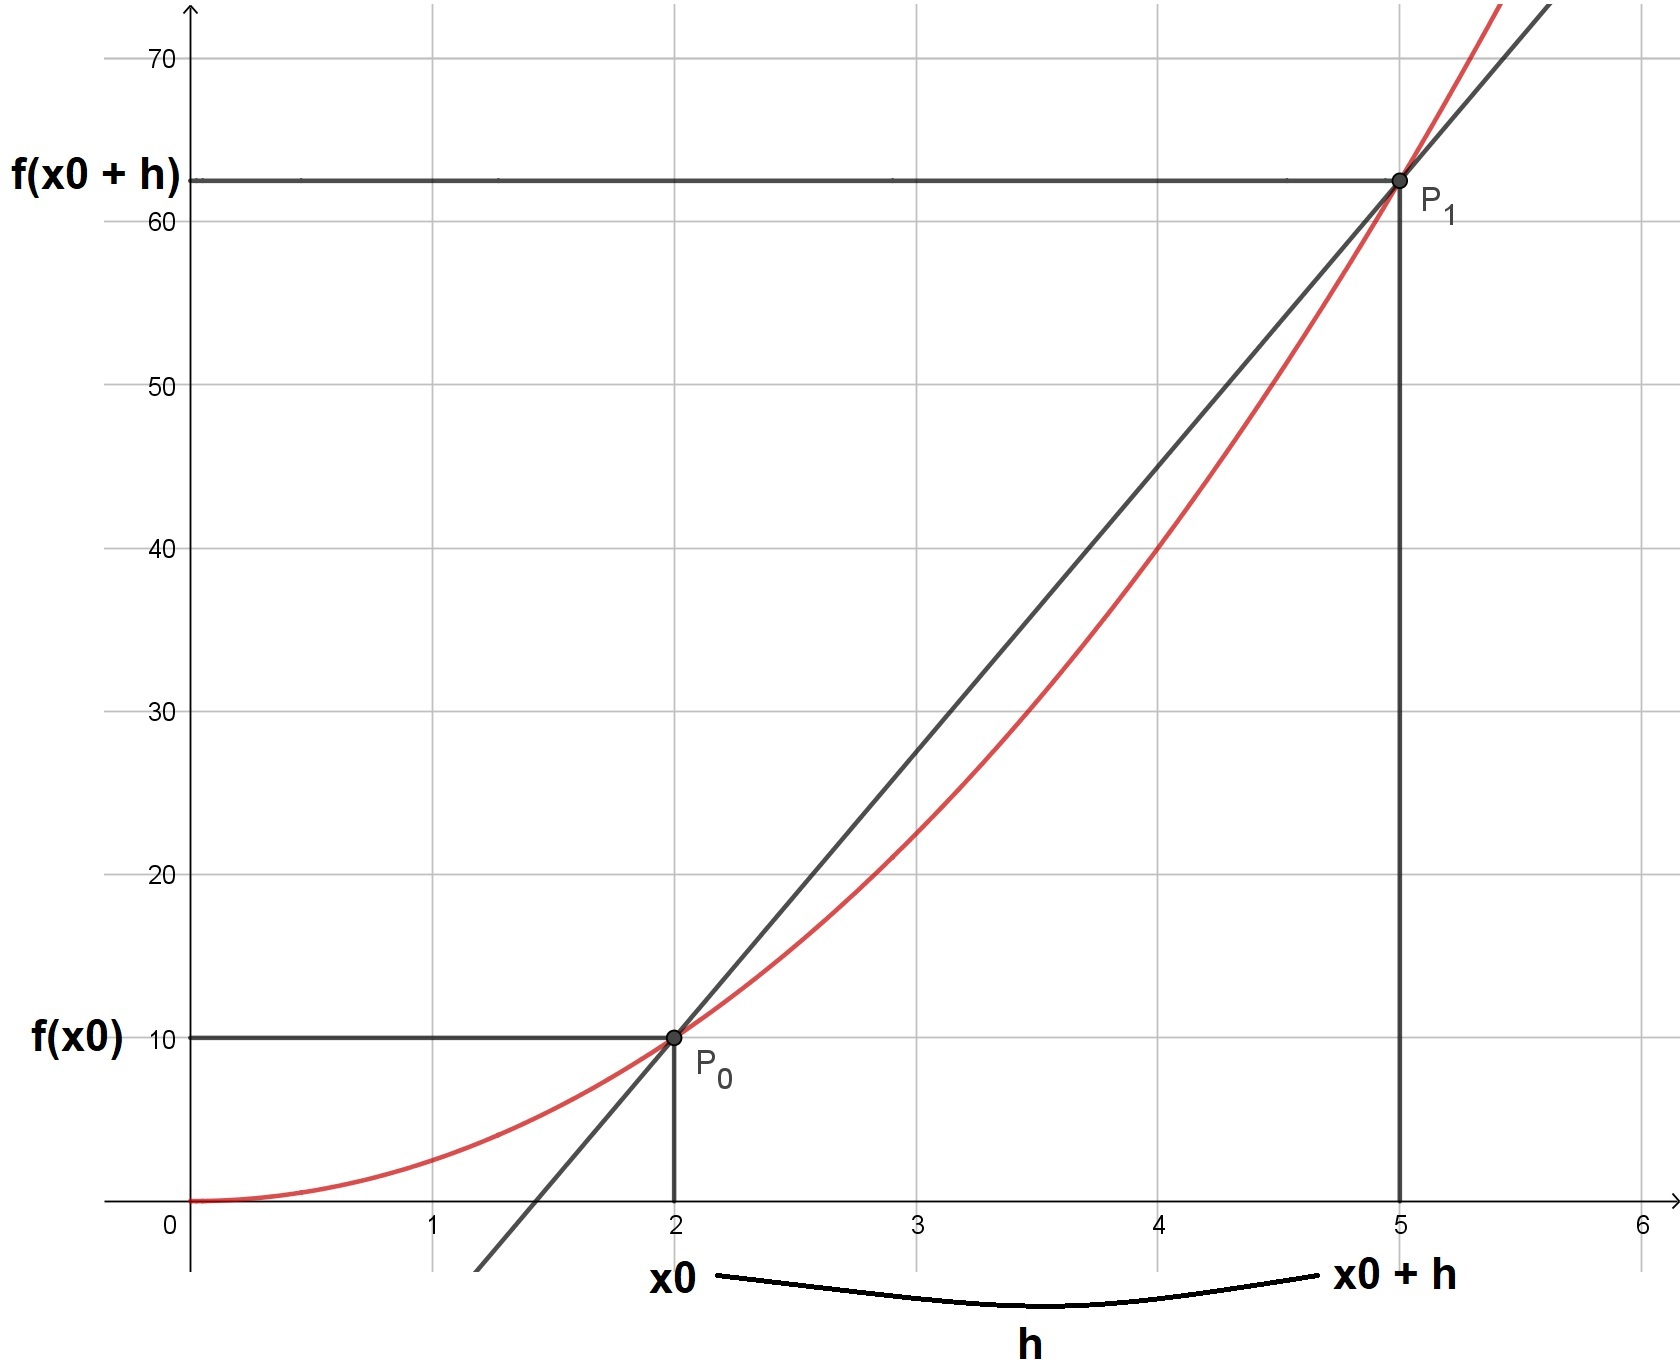
\includegraphics[width=0.45\textwidth]{../99_Bilder/04_Skr_DiffQuo.jpg}\\
		\par\noindent
		Die eingezeichnete Sekante hat die Steigung
		\[m_{[x_0;x_0+h]} = D(x_0;x_0+h) = \frac{f(x_0-h) - f(x_0)}{h}\]
		
		\rule{0.48\textwidth}{0.1pt}\\
		\par\noindent
		\texttt{Was passiert, wenn wir an h rütteln?}\\
		Schieben wir nun \(h\) in Richtung von \(x_0\), also so, dass das Intervall immer kleiner wird\footnote{\(h\rightarrow{}0\).}.\\
		\par\noindent
		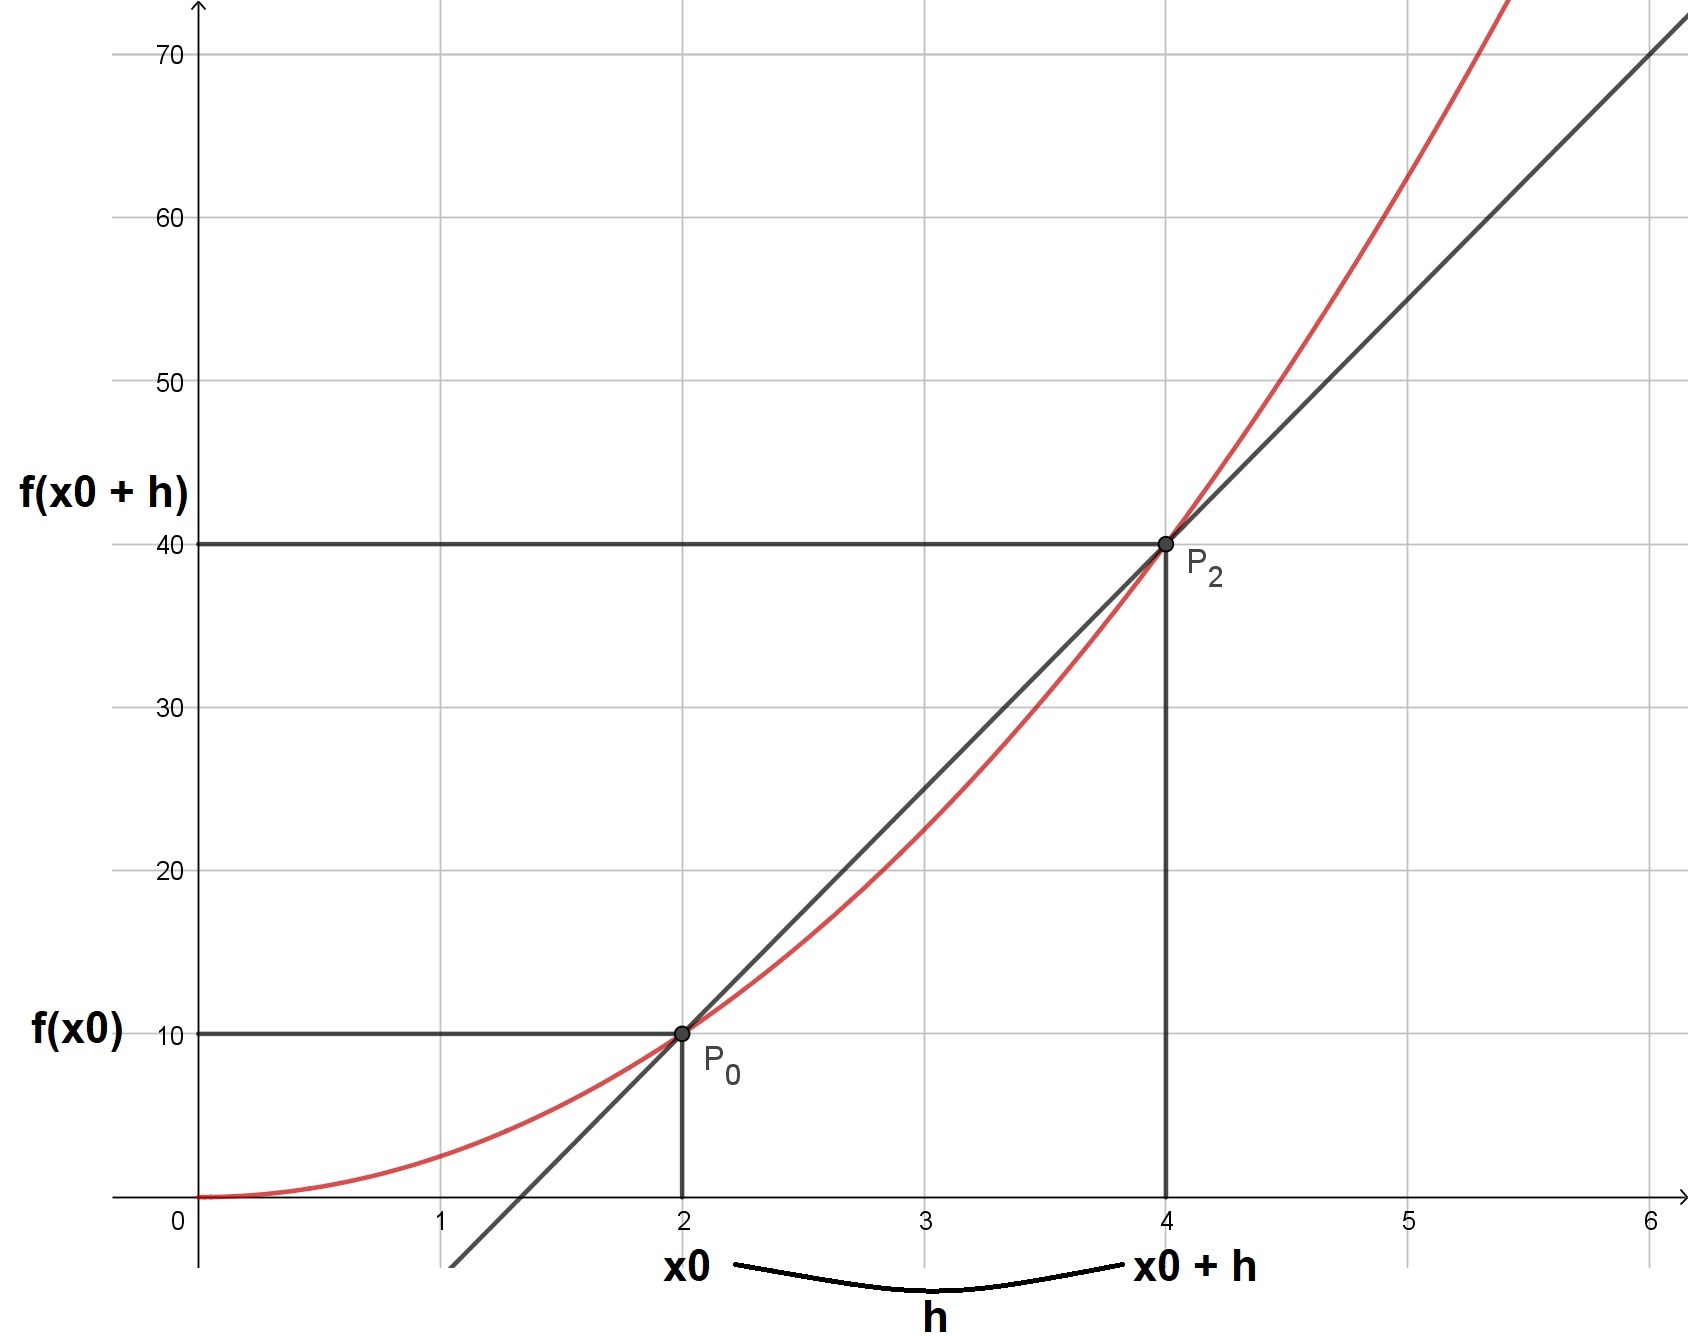
\includegraphics[width=0.48\textwidth]{../99_Bilder/04_Skr_DiffQuo_2.jpg}\\
		Schieben wir nun \(h\) immer näher an \(x_0\) ran\footnotemark[1], so wird aus unserer Sekante die Tangente im Punkt \((x_0|f(x_0))\).\\
		\par\noindent
		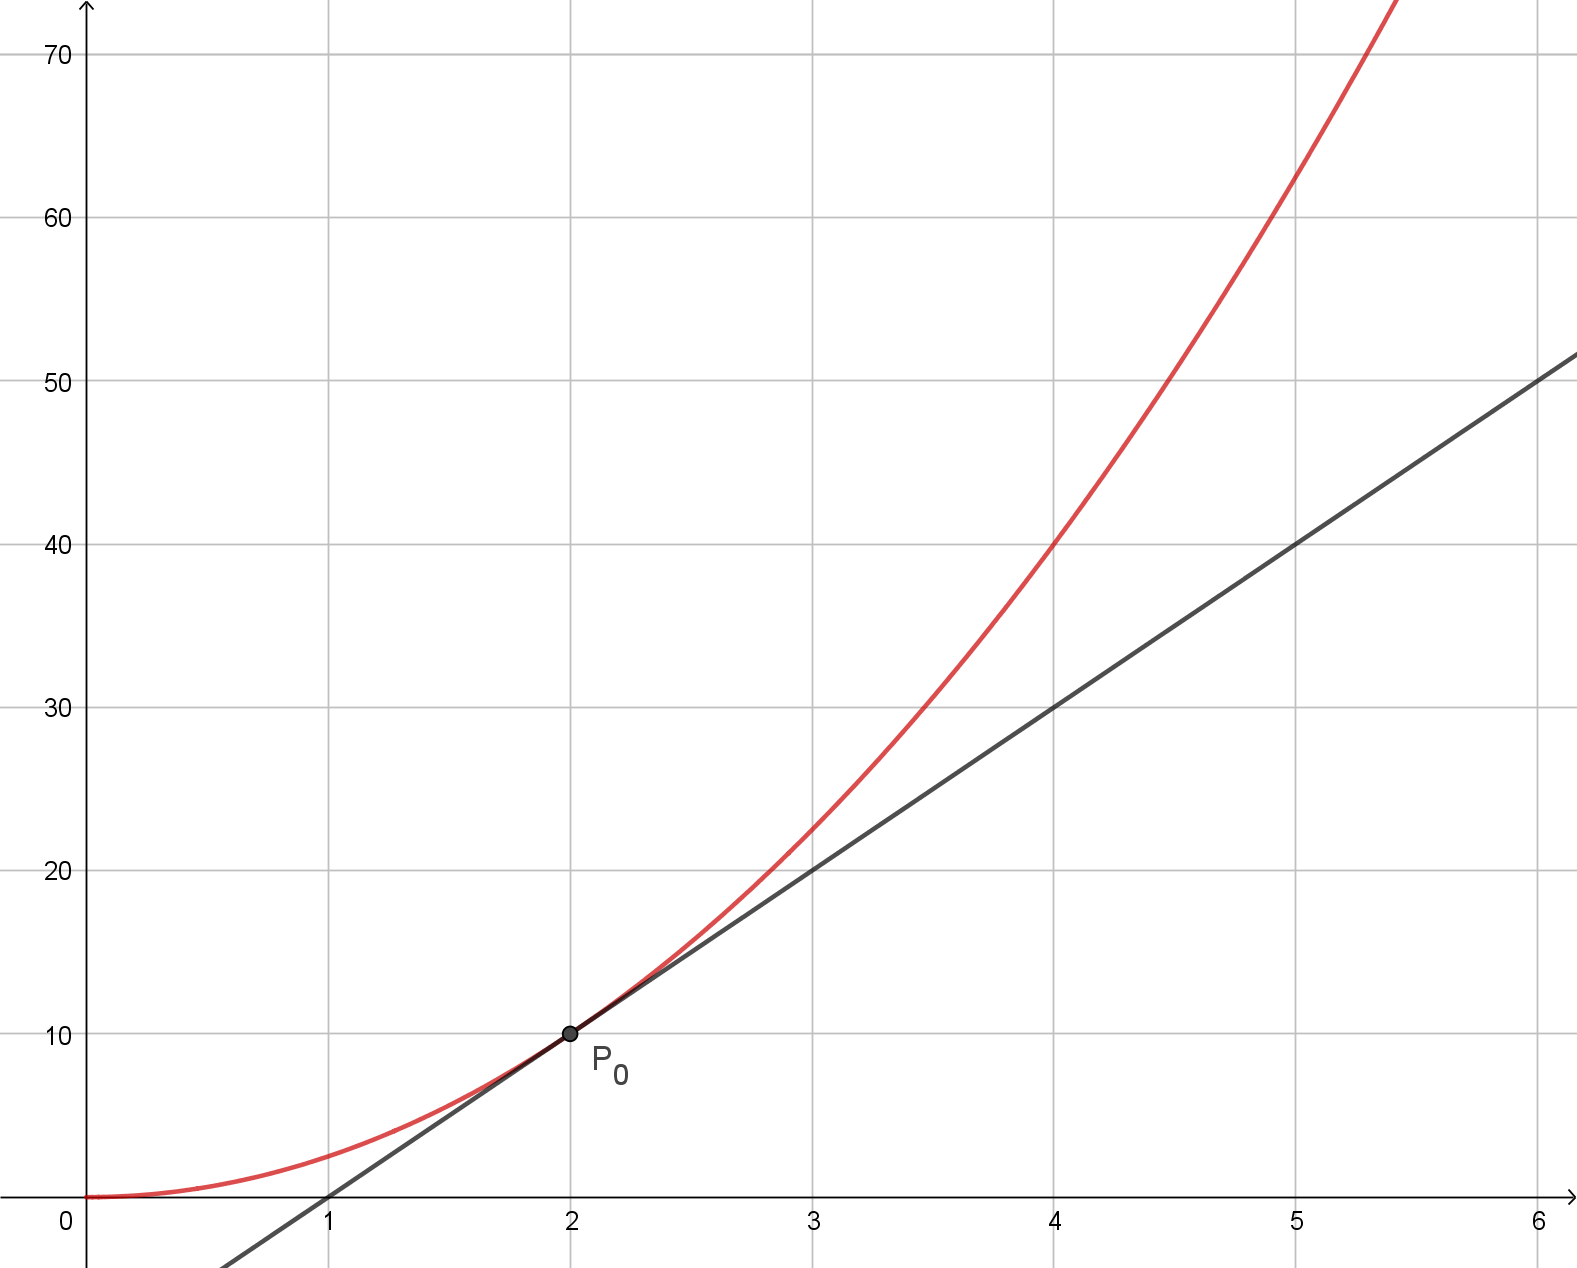
\includegraphics[width=0.48\textwidth]{../99_Bilder/04_Tang.png}\\
		\subsubsection*{Beispiel 1: Momentangeschwindigkeit an einer bestimmten Stelle}
		Beobachtet man ein Auto beim Losfahren, so kann man zu verschiedenen Zeitpunkten messen, wie viel Strecke bereits zurückgelegt wurde.\\
		Dieser Weg-Zeit-Zusammenhang lässt sich sowohl über eine Funktion \(f(x) = 2,5x^2\) wie auch über einen Graphen darstellen.\\
		\par\noindent
		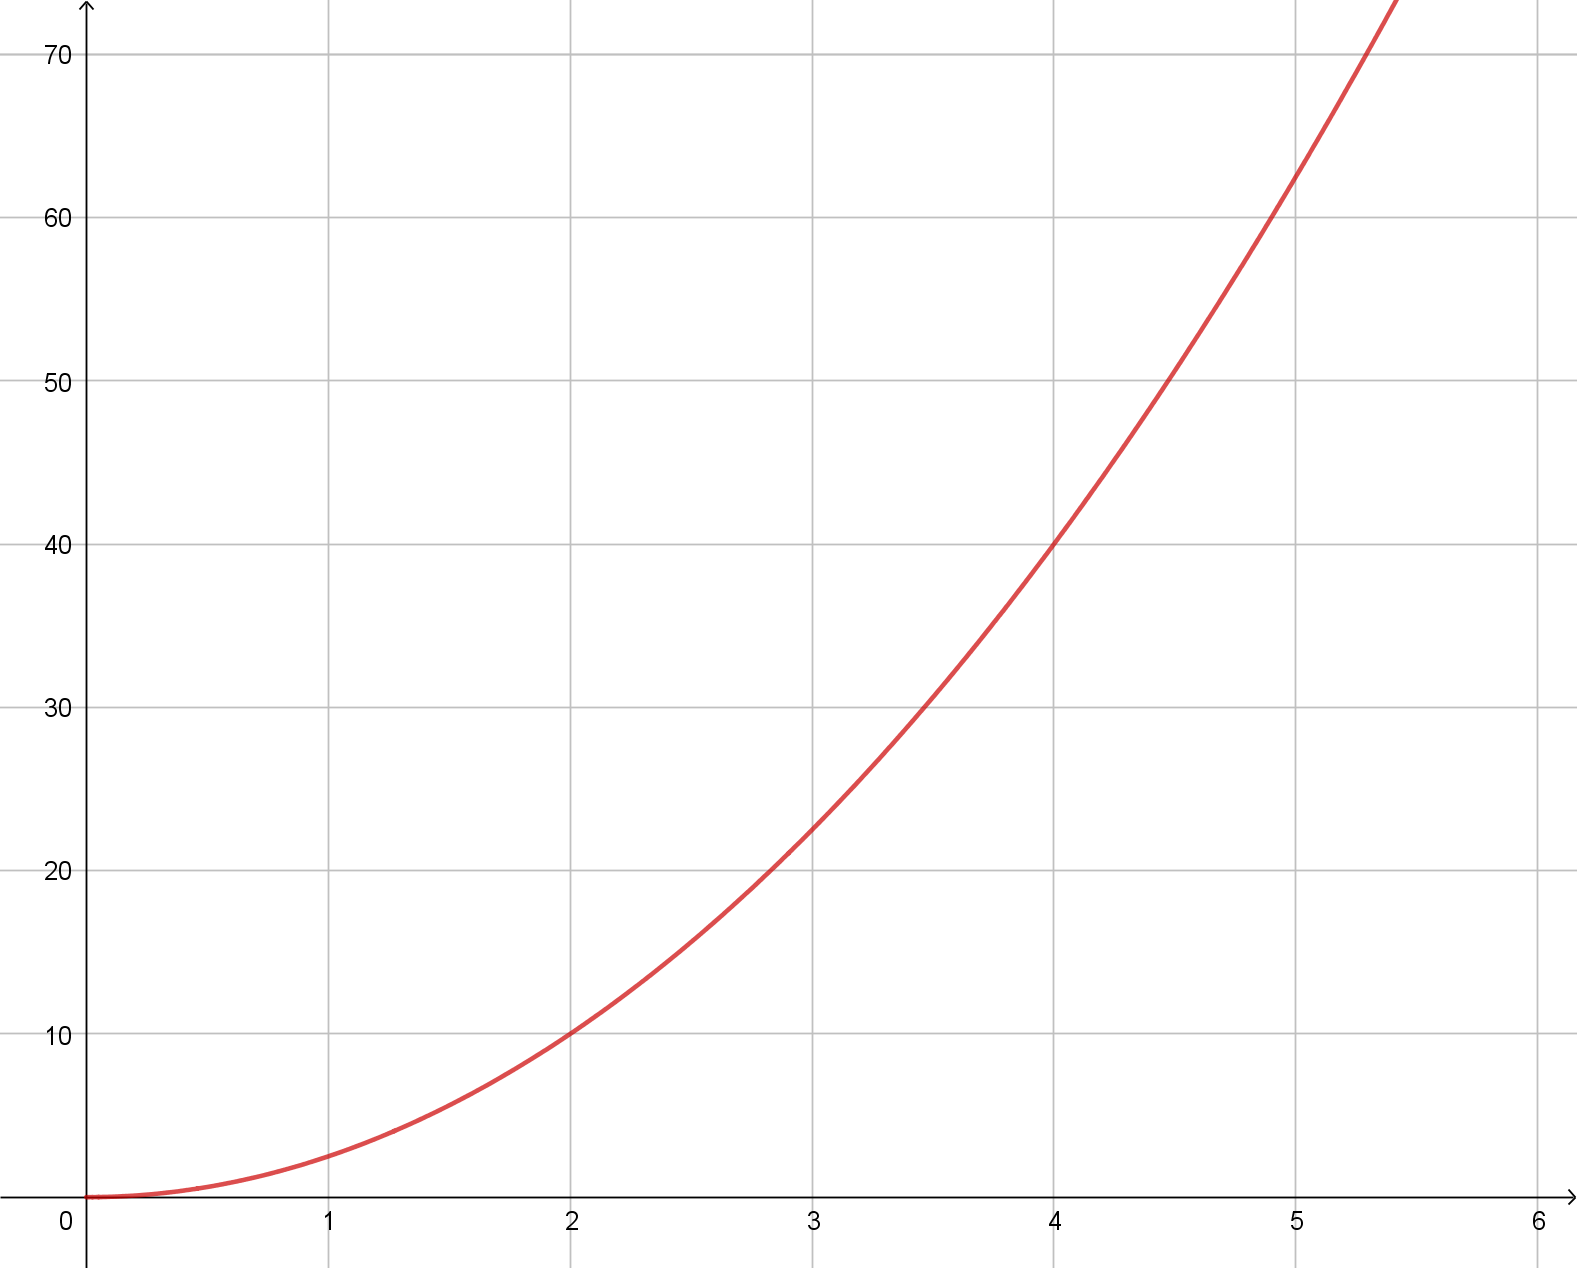
\includegraphics[width=0.48\textwidth]{../99_Bilder/04_AutoAnf.png}\\
		\par\noindent
		Wir wollen jetzt versuchen die Geschwindigkeit an der Stelle \(x_0 = 2\) zu berechnen.\\
		Zunächst wählen wir ein \(h = 3\) und berechnen den Differenzenquotient, also die Steigung der Sekante. Anschließend setzen wir \(h = 2\) und berechnen erneut den Differenzenquotient.\\
		\begin{minipage}{0.22\textwidth}
			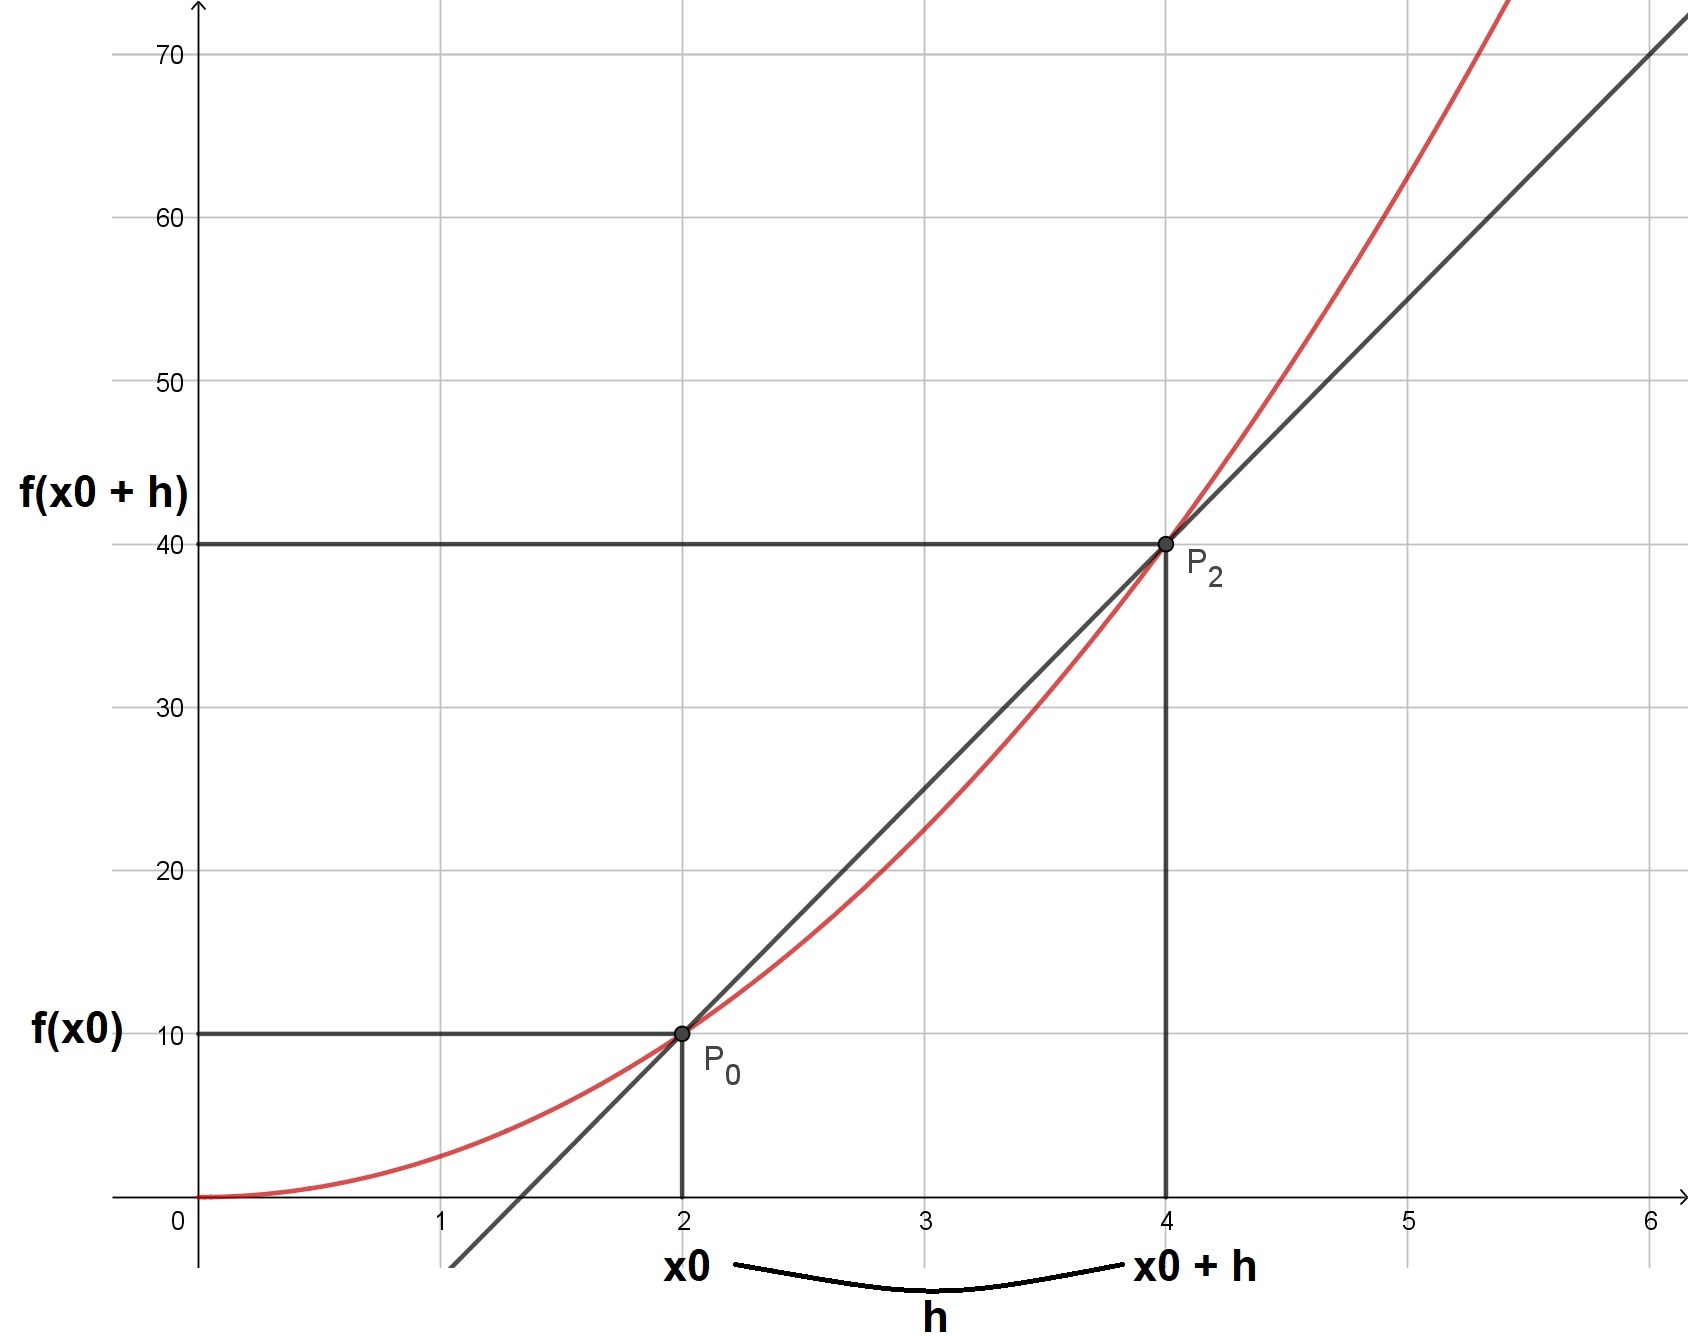
\includegraphics[width=0.98\textwidth]{../99_Bilder/04_Skr_DiffQuo_2.jpg}
		\end{minipage}
		\hfill
		\begin{minipage}{0.22\textwidth}
			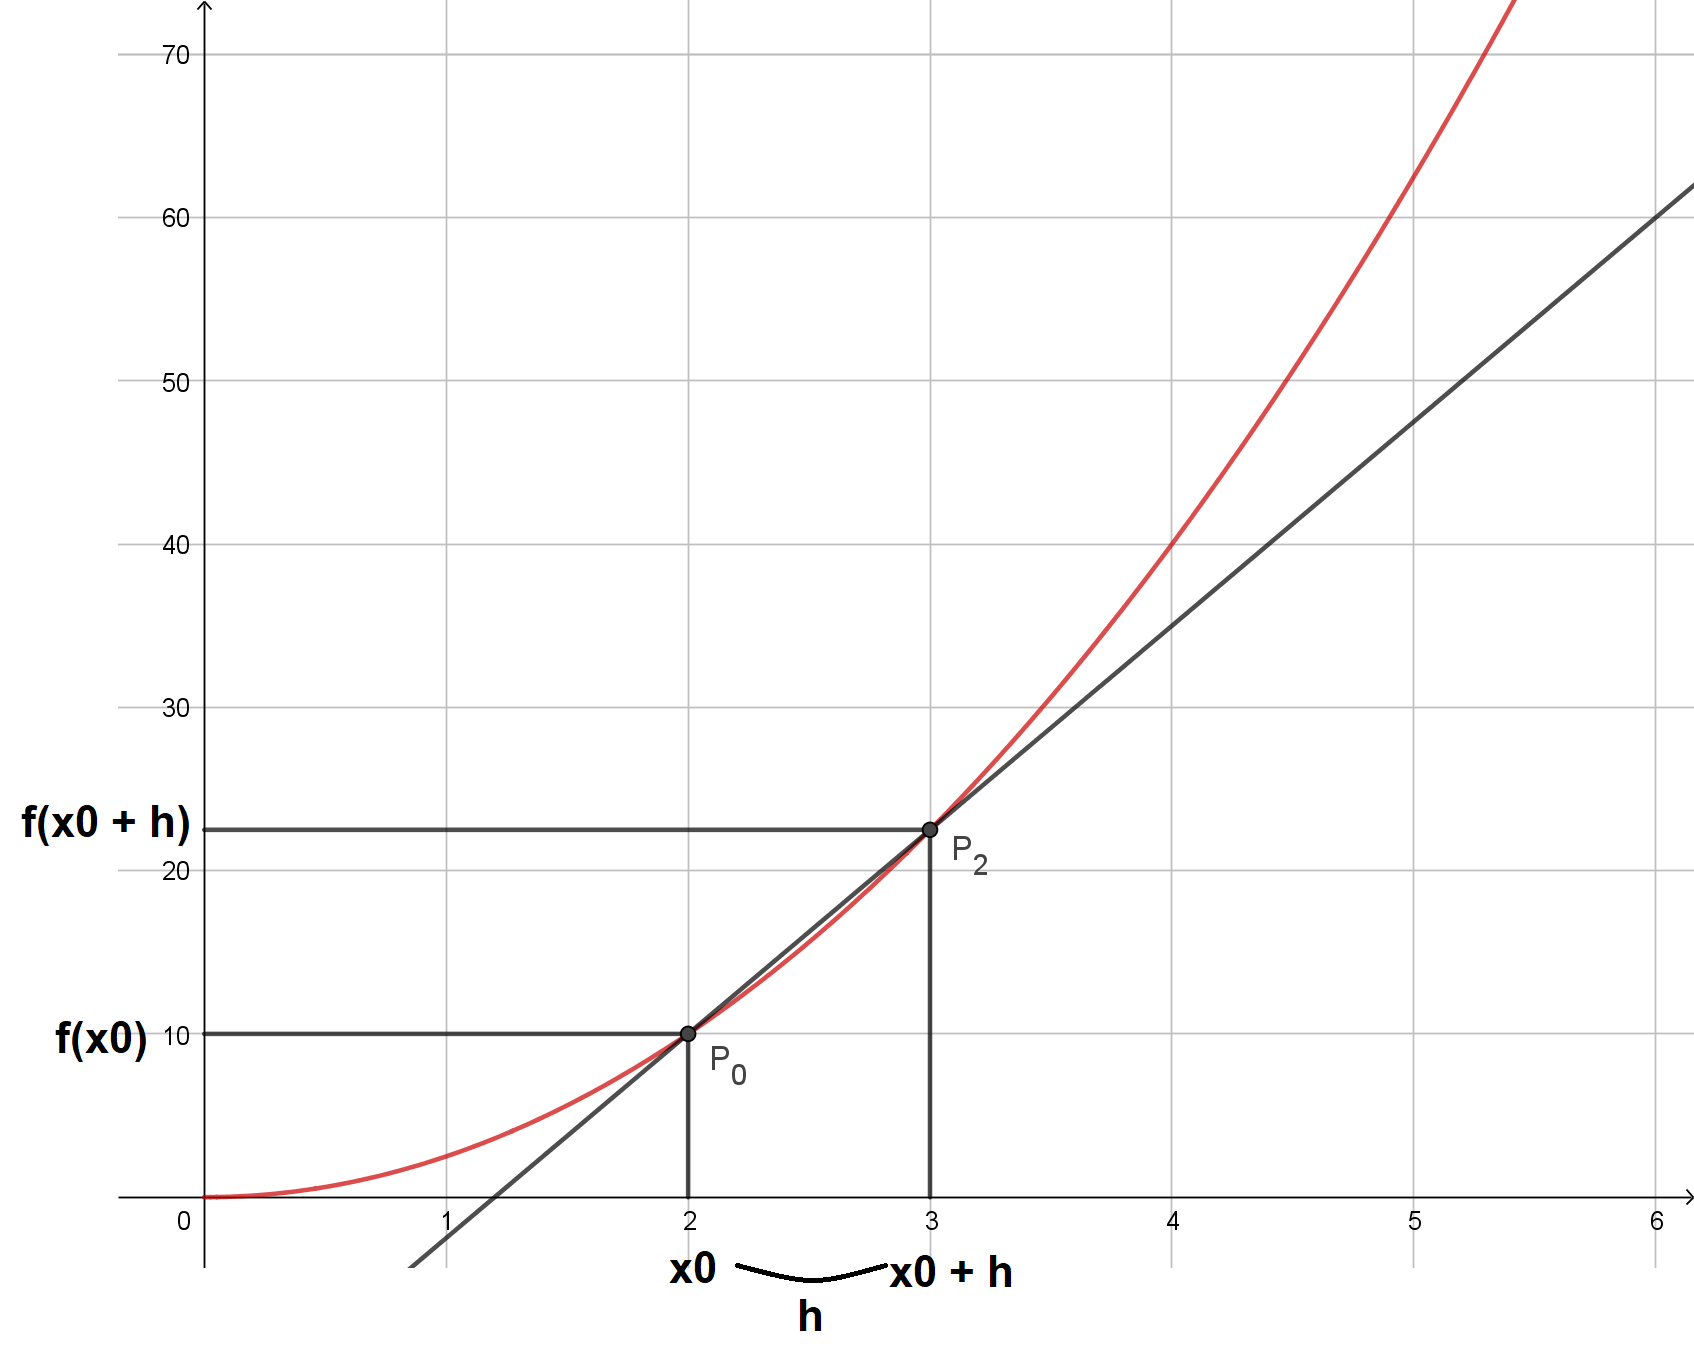
\includegraphics[width=0.98\textwidth]{../99_Bilder/04_Skr_DiffQuo_3.jpg}
		\end{minipage}
		\par\noindent
		\renewcommand{\arraystretch}{1.5}
		\begin{tabularx}{0.48\textwidth}{l|X}
			h & \(D(2;2+h) = \frac{f(2+h)-f(2)}{h}\)\\
			\hline
			\hline
			3 & \(D(2;5) = \frac{f(5) - f(2)}{3} = \frac{62,5 - 10}{3} = 17,5\)\\
			\hline
			2 & \(D(2;4) = \frac{f(4) - f(2)}{2} = \frac{40 - 10}{2} = 15\)\\
			\hline
			1 & \(D(2;3) = \frac{f(3) - f(2)}{1} = \frac{22,5 - 10}{1} = 12,5\)\\
		\end{tabularx}
		\begin{tabularx}{0.48\textwidth}{l|X}
			h & \(D(2;2 + h)\)\\
			\hline
			\hline
			0,5 & \(D(2;2,5) = \frac{f(2,5) - f(2)}{0,5} \approx \ldots \approx 11,26\)\\
			\hline
			0,1 & \(D(2;2,1) = \frac{f(2,1) - f(2)}{0,1} \approx \ldots = 10,3\)\\
			\hline
			0,01 & \(D(2;2,01) = \frac{f(2,01) - f(2)}{0,01} \approx 10,03\)\\
			\hline
			0,001 & \(D(2;2,001) = \frac{f(2,001) - f(2)}{0,001} \approx 10,003\)\\
		\end{tabularx}
		\renewcommand{\arraystretch}{1}\\
		\par\noindent
		Die Steigung an der Stelle \(x_0=2\) beträgt nach Runden \(10\).
		\par\noindent
		\hdashrule[0.5ex]{0.48\textwidth}{1pt}{3mm}
		\par\noindent
		Die Annäherung über diverse Einzelrechnungen kann sehr zeitaufwendig sein. Wir nutzen also für die Bestimmung der \textit{momentanen Änderungsrate}  bzw. der \textbf{Steigung im Punkt \(\mathbf{(x_0|f(x_0))}\)} ein Konstrukt das \textbf{Grenzwert (Limes)} genannt wird.
		\par\noindent
		\setlength{\leftskip}{0.5cm}
		\textit{Dieses Konstrukt haben wir schon beim \underline{Verhalten für große x-Beträge} kennengelernt. Dort haben wir aber \(x \rightarrow \pm\infty\) genutzt.}
		\par\noindent
		\setlength{\leftskip}{0cm}
		\rule{0.48\textwidth}{0.1pt}\\
		\par\noindent
		\texttt{Wie funktioniert das mit dem Grenzwert?}\\
		Im Prinzip kann man sich das mit dem Grenzwert so vorstellen, dass der \grq{}Zielwert\grq{} für die \grq{}wandernde\grq{} Variable eingesetzt wird.\\
		Wenn wir beispielsweise die Funktion \(f(x) = 3x^2 + 3\) haben und wissen wollen, wie die Funktion verläuft, wenn sich \(x\) an \(0\) annähert.
		\[\lim\limits_{x\rightarrow{}0} f(x) = \lim\limits_{x\rightarrow{}0} 3x^2 + 3 = 3\cdot{}0^2 + 3 = 3 \]
		\hdashrule[0.5ex]{0.48\textwidth}{1pt}{3mm}\\
		\subsubsection{Die momentane Änderungsrate mit der h-Methode}
		Genau dieses Prinzip machen wir uns also zur Bestimmung der momentanen Änderungsrate zu nutzen.\\
		Zusätzlich zu der Stelle \(x_0\), an der wir die Steigung bestimmen wollen, wählen wir einen zweiten allgemeinen Punkt \(x = x_0 + h\).\\
		Diese zwei Werte setzen wir in den Differenzenquotienten ein und setzen den Grenzwert \(\lim\limits_{h\rightarrow{}0}\)davor.
		\begin{framed}
			\noindent
			\textbf{\underline{Der Differenzialquotient}}
			\[\lim\limits_{h\rightarrow{}0} D(x_0;x_0+h) = \lim\limits_{h\rightarrow{}0} \frac{f(x_0+h) - f(x_0)}{h}\]
			gibt die \textbf{Steigung der Tangente} im Punkt \(\mathbf{(x_0|f(x_0))}\) an.\\
			\par\noindent
			Diesen \textit{Grenzwert des Differenzenquotienten} bezeichnet man als \textbf{Differenzialquotient}.
		\end{framed}
		\noindent
		Am Beispiel von eben wollen wir versuchen, den Grenzwert anzuwenden.\\
		Die Funktion lautet: \(f(x) = 2,5x^2\). Wir suchen die Steigung an der Stelle \(x_0=2\)
		\begin{align*}
			& \lim\limits_{h\rightarrow{}0} D(2;2+h)\\
			& = \lim\limits_{h\rightarrow{}0} \frac{f(2+h)-f(2)}{h}\\
			& = \lim\limits_{h\rightarrow{}0} \frac{2,5\cdot(2+h)^2 - 2,5\cdot{}2^2}{h}\\
			& = \lim\limits_{h\rightarrow{}0} \frac{2,5\cdot((2+h)^2 - 2^2)}{h}
		\end{align*}
		Wir können jetzt aber nicht einfach für \(h = 0\) einsetzen, da wir sonst durch \(0\) teilen würden.\\
		\textbf{Teilen durch \(0\) ist \underline{nicht} möglich.}\\
		Wir müssen also versuchen, das \(h\) aus dem Nenner zu kürzen.
		\begin{align*}
			& = \lim\limits_{h\rightarrow{}0} \frac{2,5\cdot(4 + 4h + h^2 - 4)}{h}\\
			& = \lim\limits_{h\rightarrow{}0} \frac{2,5\cdot(4h + h^2)}{h}\\
		\end{align*}
		\begin{align*}
			& = \lim\limits_{h\rightarrow{}0} \frac{2,5\cdot\cancel{h}(4 + h)}{\cancel{h}}\\
			& = \lim\limits_{h\rightarrow{}0} 2,5(4 + h)\\
		\end{align*}
		Jetzt können wir für \(h = 0\) einsetzen und erhalten für die Steigung des Graphen an der Stelle \(x_0=2\)
		\begin{align*}
			\lim\limits_{h\rightarrow{}0} D(2;2+h) & = 10
		\end{align*}
	\end{worksheet}
\end{document}